\documentclass[11pt]{article}
% Checkpoint report. Figures and numbers come from make_figures.py (figures/numbers.json).
% Build:  cd report && latexmk -pdf checkpoint.tex

\usepackage[margin=1in]{geometry}
\usepackage{amsmath,amssymb}
\usepackage{graphicx}
\usepackage{booktabs}
\usepackage{siunitx}
\usepackage{xcolor}
\usepackage{caption}
\usepackage{subcaption}
\usepackage{float}
\usepackage[hidelinks]{hyperref}
\usepackage[capitalise]{cleveref}

\captionsetup{font=small,labelfont=bf}
\newcommand{\KE}{\mathrm{KE}}
\newcommand{\todo}[1]{\textcolor{red!70!black}{[\textbf{TODO:} #1]}}

\title{Robust Impact Mitigation with Heterogeneous Nonlinear Metamaterials:\\
       Replicating and Extending a Discrete-Element Study\\[4pt]
       \large Checkpoint Report}
\author{\todo{author names}}
\date{\today}

\begin{document}
\maketitle

%======================================================================
\begin{abstract}
Nonlinear elastic constitutive laws, in particular bistable and snap-through springs,
can strongly attenuate the kinetic energy that an impact transmits through an
architected material, but optimized nonlinear designs are known to be highly sensitive
to small changes in material parameters and impact conditions. Tamur
\emph{et al.}~\cite{tamur} showed computationally that making the \emph{nonlinear} part
of the spring laws spatially heterogeneous improves this robustness. In this project we
replicate their study and use it as a testbed for data-driven design. We
re-implemented their one-dimensional discrete element model (DEM): a 20-mass chain with
four families of cubic-polynomial springs, struck by a light impactor. The
re-implementation is a compiled, batched Python solver that matches the authors' MATLAB
code to a median relative difference of $6\times10^{-7}$ in the performance metric and
runs about 500 simulations per second on four CPU cores. With it we reproduced the
paper's impactor-mass perturbation results (to two significant figures) and its
coefficient-noise robustness trend. We also generated a dataset of 360{,}000 simulated
designs that spans the paper's admissible design space. Preliminary sensitivity
analyses confirm the paper's central qualitative finding: homogeneous bistable chains
are the most sensitive to perturbations and heterogeneous chains without bistable
springs are the least. The next stage replaces the gradient-based inverse design of the
original work with Gaussian-process (GP) surrogate optimization.
\end{abstract}

%======================================================================
\section{Introduction}

\subsection{Background and problem statement}

Protecting a structure or a person from impact means limiting how much of the incoming
energy reaches the protected side. Material heterogeneity is known to raise damage
tolerance in quasi-static settings, as in bone and other biological
materials~\cite{keaveny,wegst}. Separately, in dynamic settings, nonlinear elastic
responses have emerged as a passive way to reshape stress waves~\cite{patil,nesterenko}.
Strong nonlinearity combined with dispersion can break an impulse into a train of
smaller solitary waves~\cite{nesterenko}, and bistable elements can trap strain energy
or dissipate it~\cite{shan,xiu}. The drawback is sensitivity. Nonlinear systems can
respond very differently to small changes in impactor condition or material
properties~\cite{strogatz}, and bistable chains can even localize and transmit
\emph{more} kinetic energy than their linear counterparts~\cite{fancher}. A design that is
optimal on paper may therefore perform poorly once manufactured.

We study the model of Tamur \emph{et al.}~\cite{tamur}. A chain of $N=20$ unit masses is
joined by springs that are linear in tension and cubic in compression, each with a
viscous damper in parallel ($\zeta=0.02$), and fixed to a wall at the far end. In
compression the spring law of family $I$ is
\begin{equation}
  f_I(\Delta x) = \Delta x + c_{2I}\,\Delta x^2 + c_{3I}\,\Delta x^3,
  \qquad I\in\{A,B,C,D\},
  \label{eq:spring}
\end{equation}
with five consecutive springs per family, so that the linear stiffness is uniform and
only the nonlinear terms vary along the chain. A point-mass impactor ($M/M_0=0.01$,
$V/V_0=0.25$, with $M_0$ half the chain mass and $V_0$ the linear sound speed) hits the
first mass through a tension-free Hertzian contact
$f_H = C_\text{imp}[x_0-x_1]_+^{3/2}$ with $C_\text{imp}=1.2\times10^4$. The performance
metric, which is also the design objective, is the \emph{KE ratio}
\begin{equation}
  \KE = \frac{\max_t \KE_{N}^{\text{non}}(t)}{\max_t \KE_{N}^{\text{lin}}(t)},
  \label{eq:ke}
\end{equation}
the peak kinetic energy of the last mass, divided by the same quantity for the purely
linear chain. Lower is better. Admissible designs satisfy
$c_2\in[-120,0]$, $c_3\in[0,4000]$ and positive strain energy,
$c_3 > \tfrac{2}{9}c_2^2$, for every family. The roots of $f$ and $f'$ split this
space into monotonic ($c_2^2\le 3c_3$), snap-through ($3c_3<c_2^2\le 4c_3$) and
bistable ($c_2^2>4c_3$) springs~\cite{tamur}.

Three design categories are compared: \emph{homogeneous} (one spring law, 2
variables), \emph{heterogeneous} (four laws, 8 variables) and
\emph{heterogeneous excluding bistability} (four laws, with $c_2^2\le 4c_3$ in every
family). \textbf{Our problem} is twofold:
(i) to reproduce, independently, the paper's evidence that heterogeneity in the
nonlinear constitutive response improves robustness to uncertainty in the spring
coefficients and impact conditions; and
(ii) to evaluate a sample-efficient, data-driven alternative to the paper's
finite-difference gradient optimizer, namely GP surrogate optimization, on this
expensive and rugged objective.

\subsection{Literature review and previous work}

\paragraph{Disorder and wave transport.}
Anderson showed that sufficient disorder can stop energy from diffusing in linear
lattices~\cite{anderson}. Related ideas have been used to widen band gaps in phononic
crystals and acoustic metamaterials~\cite{hussein}. In nonlinear lattices the effect of
disorder is less clear: depending on the case, nonlinearity has been found to
preserve, destroy or modify localization~\cite{laptyeva}.

\paragraph{Nonlinear and bistable metamaterials for impact.}
Granular and other strongly nonlinear chains convert impulses into solitary
waves~\cite{nesterenko,patil}. Multistable architected materials can trap elastic
strain energy~\cite{shan}. In bistable chains, the absorbed kinetic energy depends
non-monotonically on impactor mass and velocity~\cite{fancher}. Reducing intersite
viscosity can increase relative energy absorption, but only when the chain is finely
enough discretized~\cite{xiu}. MacNider \emph{et al.}\ used bilevel inverse design to
tailor nonlinear constitutive laws for target wave responses, and found that optimal
homogeneous designs were bistable~\cite{macnider}.

\paragraph{The replicated study.}
Tamur \emph{et al.}~\cite{tamur} optimized the coefficients $(c_2,c_3)$ of
\cref{eq:spring} with MATLAB's \texttt{fmincon} (finite-difference gradients, random
initial designs) and integrated the DEM with \texttt{ode45}~\cite{dormand,shampine}.
The best KE ratios they report are $0.56\%$ (heterogeneous), $1.17\%$ (homogeneous) and
$0.86\%$ (heterogeneous excluding bistability). They then perturbed the coefficients by
Gaussian noise of level $\epsilon\le5\%$. At $\epsilon=5\%$, the homogeneous design's
KE ratio worsened $8\times$, the heterogeneous design's $12\times$ (from a lower
baseline), and the bistability-free design's only $3\times$. Over ensembles of 200
optimized designs per category, the median perturbed KE ratio was $0.105$, $0.067$ and
$0.050$ respectively.

\paragraph{Surrogate-based optimization.}
Every KE evaluation requires two stiff, long-time ODE integrations, and the objective
landscape is rugged (\cref{fig:impact}). Gaussian-process regression~\cite{rasmussen}
with expected-improvement acquisition~\cite{jones} is a standard way to optimize such
expensive black-box functions with few evaluations. GP models also provide predictive
uncertainty, which is directly relevant to a robustness study.

\subsection{Description of the data}

All data are generated by simulation; no experimental measurements are involved.

\paragraph{Simulator.}
We ported the authors' MATLAB DEM to Python twice. The first port is a line-by-line
\texttt{scipy} version~\cite{scipy} that serves as a reference. The second is a
Numba-compiled~\cite{numba} adaptive Dormand--Prince 5(4) integrator (the same method
as \texttt{ode45} and \texttt{scipy}'s RK45) that runs one simulation per CPU thread,
stops at $T=25/f_0\approx497$, and takes the peak of $\KE_N$ continuously from the
solver's dense output. Tolerances are $\text{rtol}=\text{atol}=10^{-12}$.
\Cref{tab:validation} summarizes the verification.

\paragraph{Dataset.}
The dataset contains $360{,}000$ nominal designs, \num{120000} per category, drawn
uniformly from the admissible region by rejection sampling with seed 0. Each row holds:
\begin{itemize}\itemsep0pt
  \item \textbf{inputs}: $c_2,c_3\in\mathbb{R}^4$ for families A--D (8 features; for
        homogeneous rows all four families share one pair);
  \item \textbf{target}: the KE ratio (\cref{eq:ke}); it spans more than three decades
        (\cref{fig:data}), so we model $\log\KE$;
  \item \textbf{metadata}: category, the SI-3 spring type of each family, solver step
        count and status. All $360{,}000$ integrations succeeded.
\end{itemize}
Across all families, 84.3\% of the sampled springs are monotonic, 12.6\% snap-through
and 3.1\% bistable. Good designs are rare: only 92, 405 and 317 designs (homogeneous,
heterogeneous, excl.\ bistability) reach $\KE\le0.03$. The best random designs reach
$0.0114$, $0.0089$ and $0.0112$, versus the paper's optimized $0.0117$, $0.0056$ and
$0.0086$. The generator can also attach Monte Carlo perturbed copies of each design
(paper Eq.~4), which provides robustness labels (mean and standard deviation of $\KE$
under noise).

%======================================================================
\section{Preliminary analysis}

\paragraph{Simulator verification.}
\Cref{tab:validation} lists the checks that pass. All of them are
reproducible with the script \texttt{check\_simulation.py} in the \texttt{fast} folder. The equations of motion agree with MATLAB to
machine precision. The KE ratio agrees with MATLAB's \texttt{ode45} to a median relative
difference of $6\times10^{-7}$. For the paper's Fig.~4 case (impactor mass increased by
1\%), we reproduce every reported number. Four of the six designs tabulated in the
paper's SI agree to within 3\%. The remaining two (homogeneous optimum and heterogeneous
perturbed) contain bistable springs. Perturbing their published coefficients by less
than the $\pm0.005$ rounding of the table moves $\KE$ over $0.0117$--$0.062$ and
$0.0117$--$0.038$, and both ranges contain the paper's values. We therefore attribute
the mismatch to the printed precision, not to the model. Measuring the peak on the
paper's coarser output grid instead changes $\KE$ by less than $0.3\%$.

\begin{table}[H]
  \centering\small
  \caption{Verification of the Python DEM. Paper values are from Tamur
  \emph{et al.}~\cite{tamur} (SI Tables S1--S2 and Sec.~3).}
  \label{tab:validation}
  \resizebox{\linewidth}{!}{%
  \begin{tabular}{@{}lll@{}}
    \toprule
    Check & Ours & Reference \\
    \midrule
    Equations of motion, 5000 random states        & max diff.\ $6\times10^{-16}$ & MATLAB \\
    KE ratio, 16 designs                           & median rel.\ diff.\ $6\times10^{-7}$ & MATLAB \texttt{ode45} \\
    Heterogeneous optimum                          & 0.0057 & 0.0056 \\
    Het.\ excl.\ bistability optimum               & 0.0086 & 0.0086 \\
    Homogeneous, perturbed                         & 0.0627 & 0.062 \\
    Het.\ excl.\ bistability, perturbed            & 0.0145 & 0.015 \\
    Linear chain, $1.01M$: peak-KE increase        & $\times1.018$ & $\times1.02$ \\
    $1.01M$: KE homo / hetero / excl.             & 0.109 / 0.026 / 0.0077 & 0.11 / 0.026 / 0.008 \\
    \bottomrule
  \end{tabular}}
\end{table}

\paragraph{One-at-a-time coefficient sensitivity.}
\Cref{fig:oat} varies each coefficient of the example design from the authors' code
($c_2=[-70,-100,-5,-35]$, $c_3=[1200,2000,1500,3000]$, $\KE=0.148$) by $\pm50\%$,
one at a time. The two families nearest the impactor (A, B) dominate: changing their
$c_2$ alone moves $\KE$ between $0.047$ and $2.7$, while families C and D barely
matter. Lowering $c_3$ in A or B quickly drives the spring out of the
positive-energy region (hollow markers), where $\KE$ exceeds the linear chain by up to
$6.4\times$. The response is also strongly non-monotonic, which already signals a
rugged objective.

\paragraph{Sensitivity to impact conditions.}
\Cref{fig:impact} slices $\KE$ around the design point for the three optimized designs
of the paper (paper Fig.~2b). The homogeneous bistable chain is extremely jagged. Its
mean $|\partial\KE/\partial(M/M_0)|$ is $1405$, against $221$ (heterogeneous) and $42$
(excl.\ bistability). The corresponding values for $|\partial\KE/\partial(V/V_0)|$ are
$56$, $9.3$ and $3.1$. This reproduces the paper's ordering and magnitudes (its
Fig.~2c).

\paragraph{Sensitivity to coefficient noise.}
\Cref{fig:noise} repeats the paper's Fig.~1c with 500 perturbed samples per noise
level, $\epsilon\in[0,5\%]$. At $\epsilon=0.25\%$ the mean $\KE$ is already
$0.071$ (homogeneous), $0.015$ (heterogeneous) and $0.0091$ (excl.\ bistability). At
$\epsilon=5\%$ it is $0.087$, $0.074$ and $0.025$, close to the paper's curves. With
the paper's unrounded homogeneous optimum ($0.0117$) these are degradations of roughly
$6\times$, $3\times$, $1\times$ and $7.5\times$, $13\times$, $3\times$, compared with the
reported $6\times,3\times,1\times$ and $8\times,12\times,3\times$. The ordering at 5\%
noise is the paper's: excluding bistability is clearly the most robust.

\paragraph{Category-level robustness (preliminary).}
Following the paper's Fig.~1d protocol, we took designs from our random dataset with
nominal $\KE\in[0.01,0.03]$, balanced over four bins (20, 84 and 60 designs; too few
random designs reach the window to obtain the paper's 200), and ran 100 Monte Carlo
trials at $\epsilon=5\%$ (\cref{fig:robust}). The median of the per-design mean
$\mu_\KE$ is $0.107$ (homogeneous), $0.046$ (heterogeneous) and $0.031$ (excl.\
bistability), against the paper's $0.105$, $0.067$ and $0.050$. The fraction with
$\mu_\KE<0.03$ is 0\%, 23\% and 47\% (paper: 0\%, 0\%, 9\%). The category ordering and
the homogeneous value match. The heterogeneous sets are more robust than in the paper,
which we expect, because random designs that land in the window are not the sharp
optima produced by an optimizer. Building optimized baseline sets is the motivation for
the GP stage.

\paragraph{Data characteristics relevant to learning.}
The target is heavy-tailed and multimodal (\cref{fig:data}). The best designs lie in a
thin tail ($<0.3\%$ of samples below $0.03$), and the response is jagged at small scales
(\cref{fig:oat,fig:impact}). For a GP surrogate this suggests modeling $\log\KE$, using
a stationary kernel with short length scales or a noise term to absorb sub-resolution
roughness, and treating the snap-through/bistable boundaries as potential
discontinuities.

%======================================================================
\section{Figures}

\subsection{Sensitivity analysis}

\begin{figure}[H]
  \centering
  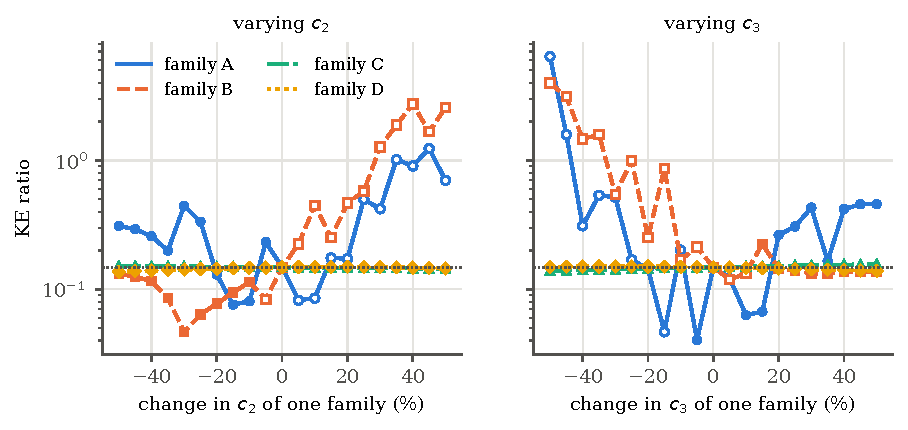
\includegraphics[width=\linewidth]{figures/oat_sensitivity.pdf}
  \caption{One-at-a-time sensitivity of the KE ratio to $c_2$ (left) and $c_3$ (right)
  of each spring family, $\pm50\%$ around the example design (dotted line,
  $\KE=0.148$). Hollow markers violate the positive-energy constraint
  $c_3>\tfrac29c_2^2$. Log scale.}
  \label{fig:oat}
\end{figure}

\begin{figure}[H]
  \centering
  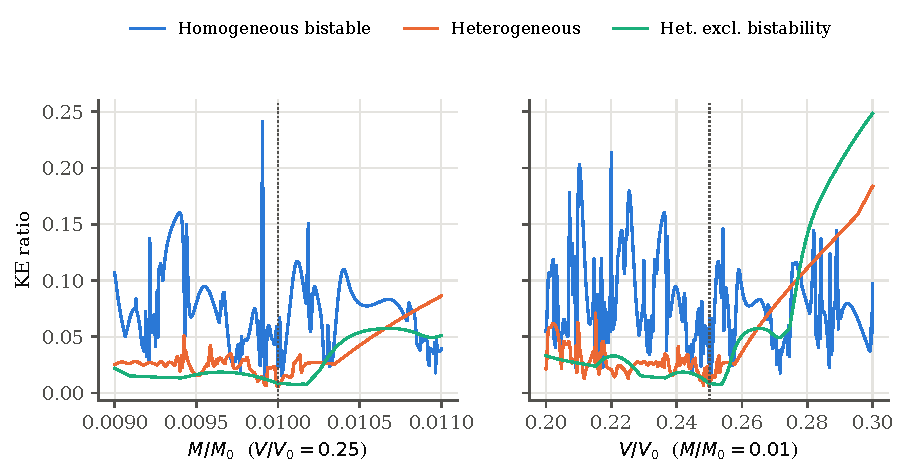
\includegraphics[width=\linewidth]{figures/impact_slices.pdf}
  \caption{KE ratio of the paper's three optimized designs along slices in impactor
  mass (left) and velocity (right) through the design point (dotted). Compare with
  Tamur \emph{et al.}\ Fig.~2b.}
  \label{fig:impact}
\end{figure}

\begin{figure}[H]
  \centering
  \begin{subfigure}[t]{0.49\linewidth}
    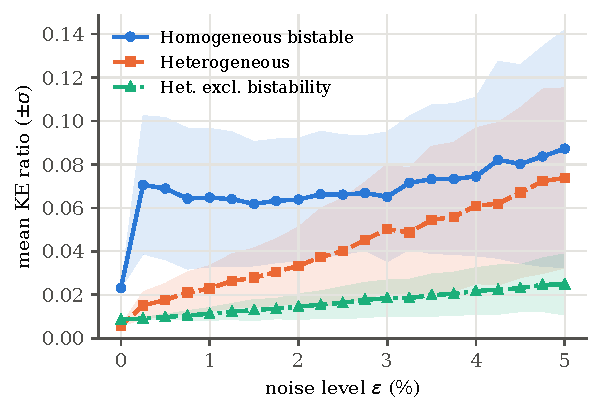
\includegraphics[width=\linewidth]{figures/noise_sweep.pdf}
    \caption{Mean $\pm$ one standard deviation of the KE ratio under Gaussian
    coefficient noise of level $\epsilon$ (500 samples per level). Compare with
    paper Fig.~1c.}
    \label{fig:noise}
  \end{subfigure}\hfill
  \begin{subfigure}[t]{0.49\linewidth}
    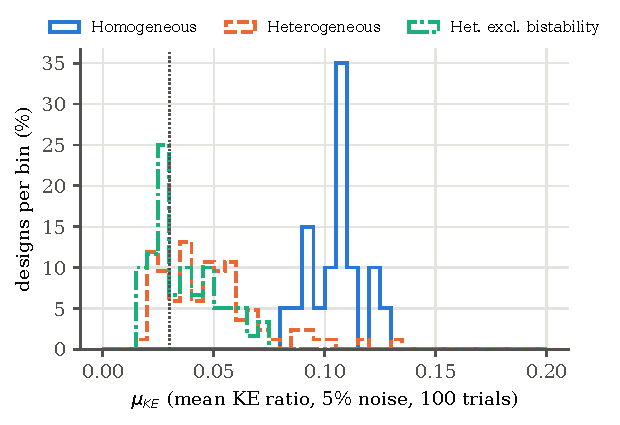
\includegraphics[width=\linewidth]{figures/robustness_prelim.pdf}
    \caption{Distribution of $\mu_\KE$ for random designs with nominal
    $\KE\in[0.01,0.03]$ after 5\% noise (100 trials each); dotted line at $0.03$.
    Compare with paper Fig.~1d.}
    \label{fig:robust}
  \end{subfigure}
  \caption{Robustness to uncertainty in the nonlinear spring coefficients.}
\end{figure}

\begin{figure}[H]
  \centering
  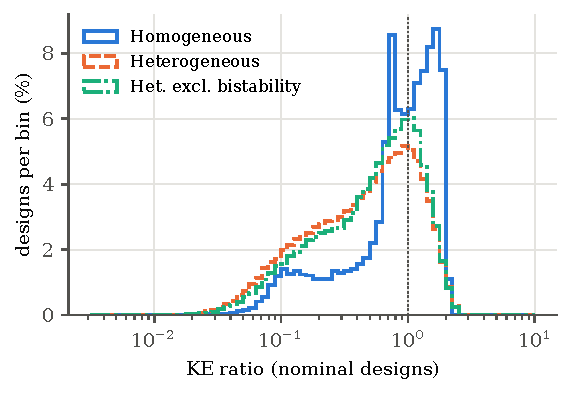
\includegraphics[width=0.6\linewidth]{figures/dataset_hist.pdf}
  \caption{Distribution of the KE ratio over the \num{360000}-design dataset, by
  category. Designs left of the dotted line outperform the linear chain.}
  \label{fig:data}
\end{figure}

\subsection{GP optimization results}

\begin{figure}[H]
  \centering
  \fbox{\parbox[c][5cm][c]{0.8\linewidth}{\centering\small
    \textbf{Placeholder: GP optimization not yet run.}\\[6pt]
    Planned panels: (a) best $\KE$ found vs.\ number of simulations, GP-EI vs.\
    random search vs.\ finite-difference gradient optimization, per category;\\
    (b) GP predicted vs.\ simulated $\log\KE$ on held-out designs;\\
    (c) optimized $(c_2,c_3)$ over the SI-3 category boundaries (paper Fig.~1e).}}
  \caption{\todo{GP surrogate optimization results (next milestone).}}
  \label{fig:gp}
\end{figure}

%======================================================================
\begin{thebibliography}{99}\small

\bibitem{tamur}
C.~Tamur, M.~Brandy, H.~A.~Kim, and N.~Boechler.
Heterogeneity in constitutive nonlinearity enhances impact mitigation robustness.
Manuscript and Supplementary Information.

\bibitem{keaveny}
T.~M.~Keaveny and W.~C.~Hayes.
A 20-year perspective on the mechanical properties of trabecular bone, 1993.

\bibitem{wegst}
U.~G.~K.~Wegst, H.~Bai, E.~Saiz, A.~P.~Tomsia, and R.~O.~Ritchie.
Bioinspired structural materials.
\emph{Nature Materials}, 14(1):23--36, 2015.

\bibitem{patil}
G.~U.~Patil and K.~H.~Matlack.
Review of exploiting nonlinearity in phononic materials to enable nonlinear wave
responses.
\emph{Acta Mechanica}, 233(1):1--46, 2022.

\bibitem{nesterenko}
V.~F.~Nesterenko.
\emph{Dynamics of Heterogeneous Materials}.
Springer, New York, 2001.

\bibitem{shan}
S.~Shan, S.~H.~Kang, J.~R.~Raney, P.~Wang, L.~Fang, F.~Candido, J.~A.~Lewis, and
K.~Bertoldi.
Multistable architected materials for trapping elastic strain energy.
\emph{Advanced Materials}, 27(29):4296--4301, 2015.

\bibitem{xiu}
H.~Xiu, R.~Fancher, I.~Frankel, P.~Ziemke, M.~Fermen-Coker, M.~Begley, and
N.~Boechler.
Minimizing finite viscosity enhances relative kinetic energy absorption in bistable
mechanical metamaterials but only with sufficiently fine discretization: a nonlinear
dynamical size effect.
\emph{Journal of the Mechanics and Physics of Solids}, 200:106105, 2025.

\bibitem{strogatz}
S.~H.~Strogatz.
\emph{Nonlinear Dynamics and Chaos: With Applications to Physics, Biology, Chemistry,
and Engineering}.
CRC Press, 2024.

\bibitem{fancher}
R.~Fancher, I.~Frankel, K.~C.~H.~Chin, M.~Abi~Ghanem, B.~MacNider, L.~S.~Shannahan,
J.~F.~Berry, M.~Fermen-Coker, A.~J.~Boydston, and N.~Boechler.
Dependence of the kinetic energy absorption capacity of bistable mechanical
metamaterials on impactor mass and velocity.
\emph{Extreme Mechanics Letters}, 63:102044, 2023.

\bibitem{anderson}
P.~W.~Anderson.
Absence of diffusion in certain random lattices.
\emph{Physical Review}, 109(5):1492--1505, 1958.

\bibitem{hussein}
M.~I.~Hussein, M.~J.~Leamy, and M.~Ruzzene.
Dynamics of phononic materials and structures: historical origins, recent progress,
and future outlook.
\emph{Applied Mechanics Reviews}, 66(4):040802, 2014.

\bibitem{laptyeva}
T.~V.~Laptyeva, M.~V.~Ivanchenko, and S.~Flach.
Nonlinear lattice waves in heterogeneous media.
\emph{Journal of Physics A: Mathematical and Theoretical}, 47(49):493001, 2014.

\bibitem{macnider}
B.~MacNider, H.~Xiu, C.~Tamur, K.~Qian, I.~Frankel, M.~Brandy, H.~A.~Kim, and
N.~Boechler.
Customizable wave tailoring nonlinear materials enabled by bilevel inverse design.
\emph{Nature Communications}, 16(1):3425, 2025.

\bibitem{dormand}
J.~R.~Dormand and P.~J.~Prince.
A family of embedded Runge--Kutta formulae.
\emph{Journal of Computational and Applied Mathematics}, 6(1):19--26, 1980.

\bibitem{shampine}
L.~F.~Shampine and M.~W.~Reichelt.
The MATLAB ODE suite.
\emph{SIAM Journal on Scientific Computing}, 18(1):1--22, 1997.

\bibitem{rasmussen}
C.~E.~Rasmussen and C.~K.~I.~Williams.
\emph{Gaussian Processes for Machine Learning}.
MIT Press, 2006.

\bibitem{jones}
D.~R.~Jones, M.~Schonlau, and W.~J.~Welch.
Efficient global optimization of expensive black-box functions.
\emph{Journal of Global Optimization}, 13(4):455--492, 1998.

\bibitem{scipy}
P.~Virtanen \emph{et al.}
SciPy 1.0: fundamental algorithms for scientific computing in Python.
\emph{Nature Methods}, 17:261--272, 2020.

\bibitem{numba}
S.~K.~Lam, A.~Pitrou, and S.~Seibert.
Numba: a LLVM-based Python JIT compiler.
In \emph{Proc.\ Second Workshop on the LLVM Compiler Infrastructure in HPC}, 2015.

\end{thebibliography}

\end{document}
